\begin{figure*}[ht]
    \centering
    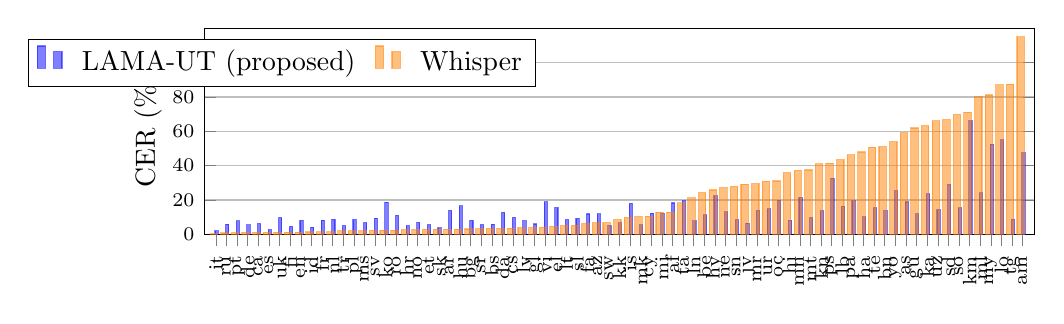
\begin{tikzpicture}
        \begin{axis}[
            width=\textwidth, 
            height=4.2cm, 
            ylabel={CER (\%)},
            ylabel style={yshift=-7pt},
            xtick={1,2,...,77}, 
            xticklabels={it, ru, pt, de, ca, es, uk, fi, en, id, fr, nl, tr, pl, ms, sv, ko, ro, hr, no, et, sk, ar, hu, bg, sr, bs, da, cs, lv, gl, vi, el, lt, sl, fa, az, sw, kk, is, mk, cy, mi, af, ta, ln, be, hy, ne, sn, jv, mr, ur, oc, hi, mn, mt, kn, ps, lb, pa, ha, te, bn, yo, as, gu, ka, uz, sd, so, km, ml, my, lo, tg, am
            },
            x tick label style={rotate=90, font=\scriptsize},
            xtick pos=bottom,
            grid=major, 
            xmajorgrids=false,
            legend style={at={(0.4,0.95)}, column sep=5pt},%, anchor=south east},
            % legend cell align={left},
            % legend style={at={(0.5, 1)},
            legend cell align={left},
            legend columns=2,
            ymin=0, ymax=120., 
            ytick={0, 20, 40, 60, 80, 100},
            y tick label style={font=\scriptsize},
            xmin=-0.1, xmax=78.1,
            ybar,
            ]
        
        \addplot+[style={blue, opacity=0.5, bar width=0.3, xshift=0.065cm}] 
            coordinates {(1, 2.0434) (2, 5.9955) (3, 7.8678) (4, 5.5343) (5, 6.3371) (6, 2.8268) (7, 9.7158) (8, 4.6651) (9, 8.1988) (10, 4.2642) (11, 8.2475) (12, 8.7417) (13, 5.1053) (14, 8.641) (15, 6.9177) (16, 9.4787) (17, 18.8081) (18, 11.0193) (19, 5.1653) (20, 6.9627) (21, 5.7385) (22, 3.802) (23, 13.936) (24, 16.6712) (25, 8.165) (26, 5.6728) (27, 5.934) (28, 12.8908) (29, 9.879) (30, 7.9353) (31, 6.0453) (32, 18.996) (33, 15.6008) (34, 8.6398) (35, 9.3782) (36, 11.8909) (37, 11.9132) (38, 5.297) (39, 6.7) (40, 18.1172) (41, 5.5156) (42, 12.3207) (43, 12.0296) (44, 18.294) (45, 19.578) (46, 7.8321) (47, 11.334) (48, 22.4033) (49, 13.1836) (50, 8.6191) (51, 6.5947) (52, 14.0207) (53, 14.906) (54, 19.8681) (55, 8.262) (56, 21.4495) (57, 9.8208) (58, 13.8512) (59, 32.7213) (60, 16.4643) (61, 19.5122) (62, 10.1785) (63, 15.4543) (64, 13.7857) (65, 25.5422) (66, 18.8821) (67, 11.9323) (68, 23.5731) (69, 14.4503) (70, 29.063) (71, 15.4388) (72, 66.2708) (73, 24.1487) (74, 52.5678) (75, 55.0304) (76, 8.8922) (77, 47.412)
            };
        \addplot+[style={orange, opacity=0.5, bar width=0.7, xshift=-0.108cm}] 
            coordinates {(1, 0.5042) (2, 0.8322) (3, 1.0532) (4, 1.125) (5, 1.1619) (6, 1.2367) (7, 1.262) (8, 1.3227) (9, 1.3455) (10, 1.4227) (11, 1.4741) (12, 1.5291) (13, 2.0229) (14, 2.0259) (15, 2.1292) (16, 2.2921) (17, 2.435) (18, 2.439) (19, 2.7453) (20, 2.7863) (21, 2.8731) (22, 2.95) (23, 2.9691) (24, 3.0123) (25, 3.1288) (26, 3.2842) (27, 3.5021) (28, 3.5785) (29, 3.6759) (30, 3.9959) (31, 4.0121) (32, 4.1578) (33, 4.7334) (34, 5.0884) (35, 5.2598) (36, 6.2866) (37, 6.8326) (38, 6.8898) (39, 8.5976) (40, 9.8542) (41, 10.3047) (42, 10.5821) (43, 12.9372) (44, 12.9688) (45, 18.3992) (46, 21.3185) (47, 24.3413) (48, 25.8559) (49, 27.2432) (50, 27.9583) (51, 29.2573) (52, 29.5538) (53, 30.9432) (54, 31.085) (55, 35.9342) (56, 37.2523) (57, 37.4938) (58, 41.0351) (59, 41.4955) (60, 43.4683) (61, 46.3415) (62, 47.9747) (63, 50.7616) (64, 51.0178) (65, 53.9499) (66, 59.2416) (67, 61.9198) (68, 63.2461) (69, 66.0443) (70, 66.866) (71, 69.925) (72, 71.1143) (73, 80.2781) (74, 81.1047) (75, 87.0318) (76, 87.4952) (77, 115.0166)};
        
        \legend{LAMA-UT (proposed)\qquad, Whisper}
        \end{axis}
    \end{tikzpicture}
    \caption{CER comparison between \shortname~and Whisper}
    \label{fig:histogram}
\end{figure*}
